\section{Long--Short Performance Heatmap}
\label{app:ls-heatmap}

Figure~\ref{fig:ls-heatmap-app} summarizes the long--short Q1$-$Q5 portfolio metrics across model--objective pairs, complementing the compact main-text Table~\ref{tab:longshort} and the extended metrics in Table~\ref{tab:ls-extended}.
Compared with the Q1 heatmap, this view emphasizes whether the full ranking separates winners from losers rather than merely selecting a strong top basket.

\begin{figure}[H]
  \centering
  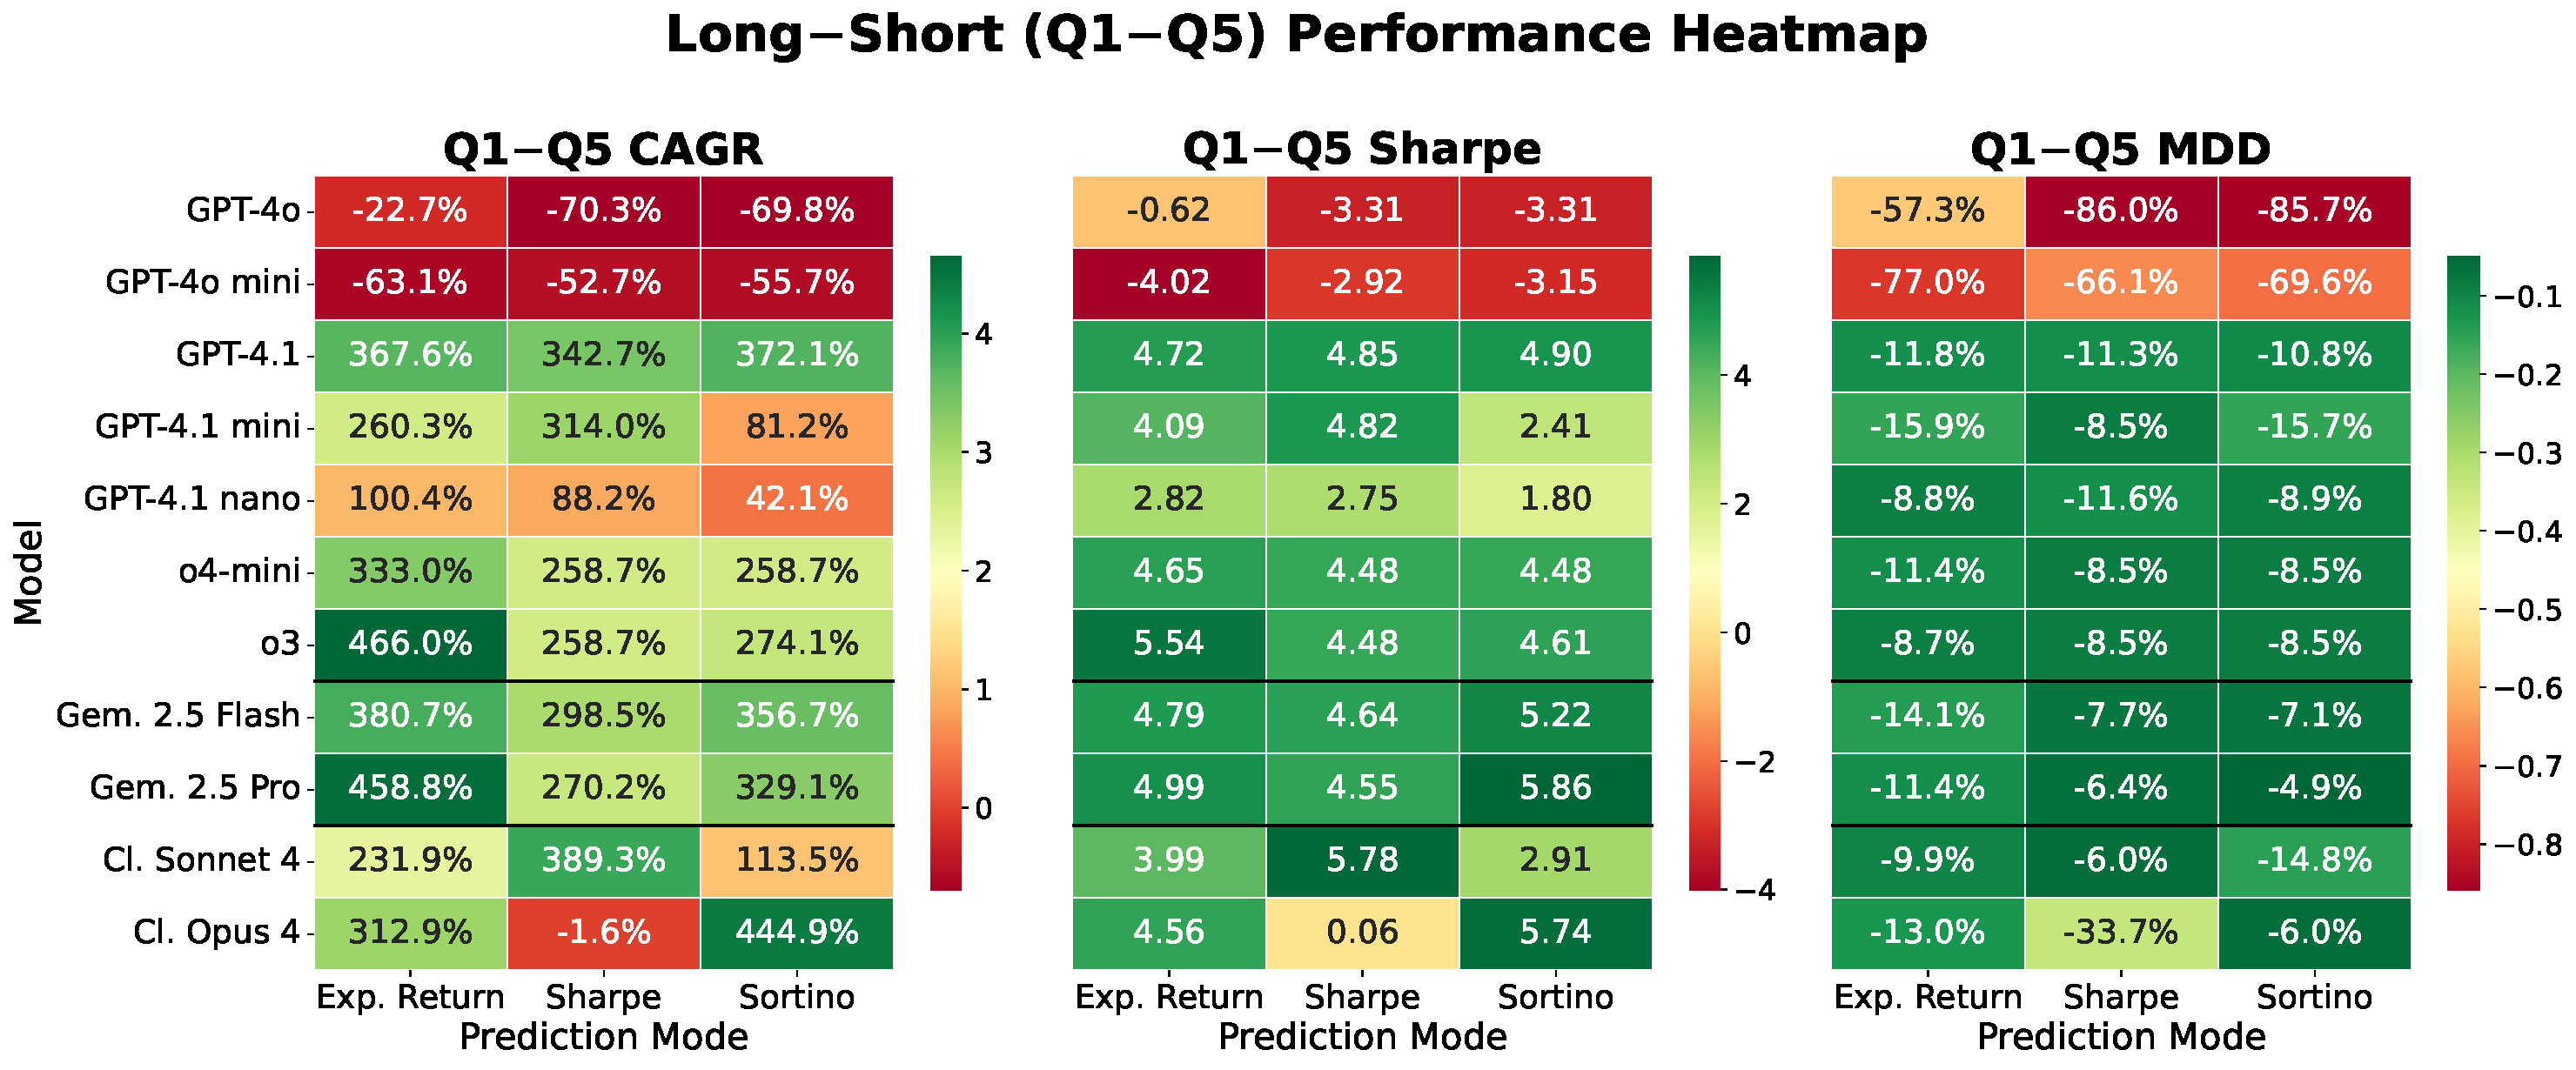
\includegraphics[width=\textwidth]{figures/fig8_longshort_performance_heatmap.pdf}
  \caption{Performance heatmap of Q1$-$Q5 long--short portfolios by model and prediction mode. Green indicates stronger values; MDD is inverted.}
  \Description{Heatmap of long-short CAGR, Sharpe, and maximum drawdown by model and prompt objective, with green indicating stronger performance and red indicating weaker performance.}
  \label{fig:ls-heatmap-app}
\end{figure}

This view is the closest appendix counterpart to the main economic test.
The strongest cells combine high spread returns with manageable drawdowns, while the weakest models show that an LLM can be systematically wrong rather than merely noisy.
The contrast with Figure~\ref{fig:q1-heatmap} helps separate market exposure from true cross-sectional ordering.

% ──────────────────────────────────────────────────────────────
\clearpage
